% Harsanyi transformation: Nature moves first, Row cannot tell
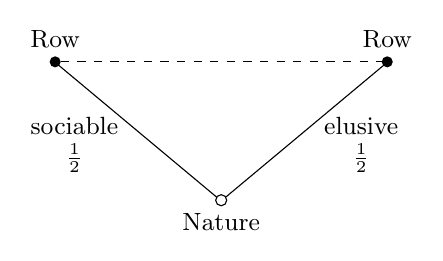
\begin{tikzpicture}[x=1pt, y=1pt, every node/.style={inner sep=1pt, font=\small}]
  \node[anchor=south] at (100,0) {Nature};
  \draw (100,12) circle (2);
  \draw (98.5,13) -- (41,61);
  \draw (101.5,13) -- (159,61);
  \node[anchor=east, align=center] at (64,32) {sociable\\$\frac{1}{2}$};
  \node[anchor=west, align=center] at (136,32) {elusive\\$\frac{1}{2}$};
  \fill (40,62) circle (2);
  \fill (160,62) circle (2);
  \draw[dashed] (42,62) -- (158,62);
  \node[anchor=south] at (40,66) {Row};
  \node[anchor=south] at (160,66) {Row};
\end{tikzpicture}
